\documentclass[letterpaper]{article}
\usepackage{polyglossia, fontspec}
\usepackage{amsmath, mathtools}
\usepackage{hyperref}
\usepackage{tikz}
\usepackage[margin = 1.5 in]{geometry}

\title{A Statistical View on the Monoallelic Expression Study}
\author{Attila G.K.}
\bibliographystyle{plain}

\begin{document}

\maketitle

\section{Rationale}

In my understanding, the aims of the project\footnote{working title: Novel
monoallelically-expressed genes and relaxation of imprinting with advanced age
in the dorsolateral prefrontal cortex.  See the text of manuscript
\href{https://docs.google.com/document/d/1cWd4UH98SJR5lihDihC0ZO-C_A1-8MQ5COcixxCLzHE/edit?usp=sharing}{under
this link}
and the corresponding figures
\href{https://docs.google.com/presentation/d/1YvpA1AJ-zzir1Iw0F25tO9x8gkSAzqaO4fjB7K3zBhE/edit?usp=sharing}{here}}
may be summarized as
\begin{enumerate}
\item classify (addressable) genes as mono or biallelically expressed in human DLFPC
\item investigate dependence on explanatory variables like age (regression)
\item estimate the fraction of monoallelically expressed genes 
\end{enumerate}

Some shortcomings (listed below) of the used approaches appear to hinder interpretation of results or
weaken the conclusions already drawn from those.
\begin{itemize}
\item implicit specification of statistical models and underlying assumptions
\item no model checking/comparison of alternative models
\item no error rates were calculated for the detection of monoallelic expression
\item consequently, only a semi-quantitative statement could be made on the
small fraction of monoallelically expressed genes
\end{itemize}

\section{Preliminaries}

Genome-wide observations on $m$ genes are based on post mortem tissue samples from the DLPFC
(dorsolateral prefrontal cortex) of $n$ individuals. The $n \times p$ design
matrix $X$ contains observations on all individuals and $p$ \emph{explanatory variables} including age of death and psychological condition (e.g.
schizophrenia).

For each gene $g$ and individual $i$ inferred to be heterozygous for \(g\) a
statistic $S_{ig}$ was derived from the SNP-array and RNA-seq data based on
read counts that contain any of the inferred SNPs in the \((i,g)\) pair.  Let
\(N_{ig}\) be the total number of such counts (based on both alleles) and
\(H_{ig} = \sum_{s} H'_{is}\), where \(H'_{is}\) is the greater of the read
counts for the two variants at SNP \(s\); the summation runs over all inferred
SNPs \(s\) (for individual \(i\) and gene \(g\)).  Using the notations just
introduced, the definition in the manuscript
reads
\begin{eqnarray*}
\label{eq:S}
S_{ig} = \frac{H_{ig}}{N_{ig}}.
\end{eqnarray*}

In this note I follow the previous analysis in that I assume
that given $X$ the random variables $\{S_{ig}\}_{ig}$ are sufficient
statistics for the parameters $\theta$ (including the level of allelic
exclusion) of all model structures under consideration.  This admittedly false
but attractively simple assumption means that the complete data (from the
SNP-array and RNA-seq measurements) carry no more information on $\theta$ than
$\{S_{ig}\}_{ig}$ do, so it is sufficient to draw inferences solely from the
latter (in combination with $X$, if $X$ is informative).  I will not discuss
sufficiency of $\{S_{ig}\}_{ig}$ further in this document.

\section{Towards explicit model specification}

To make the implicit model specification of the manuscript explicit, I will briefly expose here a
few plausible model families.  I will start from the simplest one, progressing towards generalized
linear models.  Along the way I will list mechanistic/biological assumptions behind that model, and
sketch various modeling directions to relax some of those assumptions.

\subsection{The simplest model}

For all the model families considered here the following assumptions are made
on the mechanism of allelic exclusion
\begin{itemize}
\item $\{S_{ig}\}$ are sufficient statistics (see above) for $\theta$
\item individuals are independent of each other
\end{itemize}

In case of the simplest model family, $\{S_{ig}\}$ are independently
distributed according to two likelihood functions $f(\cdot|a)$ and
$f(\cdot|b)$, corresponding to mono and biallelic expression, respectively:
\begin{eqnarray}
\label{eq:two-level}
\{S_{ig}\}_{ig} &\overset{i.i.d.}{\sim}& f(s | \theta_g) \\
\label{eq:two-level-cases}
\theta_g &=&
\begin{dcases*}
a & when $g$ is monoallelically expressed \\
b & when $g$ is biallelically expressed.
\end{dcases*}
\end{eqnarray}

For this model framework the following additional assumptions must be made on
allelic exclusion:
\begin{enumerate}
\item it takes only two levels (resulting in fully biallelic or monoallelic
expression) of the same alleles in all cells on which the data are based on
\item all genes $g$ are independent
\item $X$ has no impact (i.e.~age independence)
\end{enumerate}

\subsection{Directions for generalization}
\label{sec:generalizations}

When assumption 1 above is relaxed to allow \emph{multiple levels of allelic exclusion}
within single cells and/or variation among cells, there is a separate
$\theta_G$ parameter for each level, expressing the strength of allelic
exclusion:
\begin{equation*}
\{S_{ig}\}_{ig} \overset{i.i.d.}{\sim} f(s | \theta_G) \quad \forall g \in G.
\end{equation*}
The difficulty with this model family is twofold.  First, the biological
significance of different levels of $\theta_G$ seems vague.  Second, the
extent of monoallelic expression (genome-wide or restricted to addressable
genes) cannot be expressed by a single number such as the expected
frequency $\hat{\pi}_\mathrm{m}$ of monoallelically expressed genes that is applicable
to the two level case.  Here I will not pursue this direction further and
continue by assuming two levels as before.

\emph{Dependence among genes} (see assumption 2.) is known to exist because of extensive epigenetic
marks for imprinting spanning multiple neighboring genes.  The simplest model
family for such dependence is a HMM framework.  Emission probabilities for
\(\theta_{ig}\rightarrow S_{ig}\) are specified by \(f(s | \theta_{ig})\)
(cf.~Eq.~\ref{eq:two-level}), and
the hidden Markov chain is
\(\theta_{i1}\rightarrow\theta_{i2}\rightarrow...\), where each
\(\theta_{ig}\) may only take the two values as in
Eq.~\ref{eq:two-level-cases}.  Neither this direction is followed further
here and I return to the independent genes scenario.

Until this point \(\{S_{1g},...,S_{ng}\}\) were distributed identically and
independently across individuals for any given gene \(g\).  That allows
aggregating \(\{S_{1g},...,S_{ng}\}\) by taking the average
\(\bar{S}_g=n^{-1}\sum_i S_{ig}\), which results an estimator whose standard
error is diminished by \(n^{-1/2}\) relative to \(S_{ig}\).  Given $n=579$
this is a great improvement, yet the previous analysis did not take advantage
of this.

\subsection{Regression models}
\label{sec:regression-models}

The following regression framework achieves a similar effect to averaging.
Importantly, it also allows \(X\) to \emph{impact allelic exclusion}
(assumption 3.).  The most simple model family in this case is normal linear
regression.  Let \(f(\cdot|\mu,\sigma^2)\) denote the p.d.f.~of the normal
distribution with mean \(\mu\) and variance \(\sigma^2\).  Then for a given
individual \(i\)
\begin{eqnarray}
\label{eq:normal-lm}
\{S_{ig}\}_g &\overset{i.i.d.}{\sim}& f(s | x_i \beta_g, \sigma^2_g) \\
\label{eq:shared-regression-param}
\beta_g,\sigma^2_g &=&
\begin{dcases*}
a_1, a_2 & when $g$ is monoallelically expressed \\
b_1, b_2 & when $g$ is biallelically expressed,
\end{dcases*}
\end{eqnarray}
where \(x_i\) is the \(i\)-th row of \(X\) and \(\beta_g\) is a \(p\)-length
vector of regression coefficients.

In this model family the multi level explanatory variables \(x_i\) enter the model specification as
scaling factors of the regression parameters \(\beta_g\).  Therefore \(S_{jg}\) may be distributed
according to (many) more distributions than just two because \(f\) in Eq.~\ref{eq:normal-lm}
incorporates \(x_i\).  Yet, this model family does support binary classification since \(X\) is known
and, as in Eq.~\ref{eq:two-level-cases}, the unknown parameter(s) may only take two values.

Linearity and normal distribution may not hold\footnote{In fact they cannot exactly hold given
theoretical considerations such as the boundedness or discrete nature of \(S_{jg}\).  Despite this,
they may hold approximately well in some sense.} for \(S_{jg}\) and \(X\).  Generalized linear model
families (among which normal linear models comprise just one family) may offer solutions then.  In
this more general model family Eq.~\ref{eq:normal-lm} modifies to \(\{S_{ig'}\}
\overset{i.i.d.}{\sim} f(s | \theta_{g'}(x_i), \phi_{g'})\), such that \(\theta_{g'}\) is a function
of the explanatory variables \(x_i\), and \(g(\mathrm{E}[S_{ig'}]) = x_i \beta_{g'}\), where \(g\)
is a link function.

\subsection{The model family used in the project}

The manuscript describes the used model in bits of varying details, using two
different sets of interrelated summary statistics, in the context of different
sets of genes and different tasks.  Some details only turn out from the
scrutiny of related R code\footnote{I received Ifat's code from Andy via email
on 2/4/16}.

Taken together, the following model framework emerges (summarized in
Table~\ref{tab:model-used}):
\begin{itemize}
\item two levels of allelic exclusion: monoallelic and biallelic expression (well suited for binary classification)
\item for biallelic expression it is not clear (for me) that a model was
specified at all during the course of the study;
a confidence interval is mentioned on p6 of the manuscript but that appears to refer to distributions
of read counts instead of those of \(\{S_{ig}\}_{ig}\)
\item since
the manuscript leaves the likelihood function \(f\) unspecified and mentions
none of the generalizations of Section~\ref{sec:generalizations}
and~\ref{sec:regression-models}, I assume that the simplest model
(Eqs.~\ref{eq:two-level}-\ref{eq:two-level-cases}) describes best the
intentions of the manuscript
\item for monoallelic expression a normal linear model was used\footnote{implemented in the
\texttt{glm} R function, which was called in Ifat's code without
\texttt{family} argument thus defaulting to \texttt{gaussian}, which is the
normal linear model family. }, not on \(\{S_{ig}\}_{ig}\), but instead on a ``loss of imprinting'' statistic LOI\_R,
which I rename here to \(T_i\) to emphasize that each \(T_i\) is specific to 
individual \(i\).  \(T_i\) aggregates \(\{S_{ig}\}_{ig}\) for a few (8) genes classified
as monoallelically expressing
\item the definition of \(T_i\) is essentially
\begin{equation}
\label{eq:T}
\frac{1}{2}\left(\sum_{g=1}^8 \hat{F}_g(s) + 1 \right)
\end{equation}
where \(\hat{F}_g\) is the empirical cumulative distribution function
(e.c.d.f.) based on \(\{S_{ig}\}_i\) for one of the 8 selected genes \(g\);
thus Eq.~\ref{eq:T} gives the average e.c.d.f.~whose range is scaled to
\([0.5,1]\) to match the same interval of possible values \(S_{ig}\) may take
\end{itemize}

\begin{table}[t]
\label{tab:model-used}
\begin{center}
\begin{tabular}{c|c|c|}
statistic & \(S_{ig}\) & \(T_i\) (=LOI\_R) \\
\hline
definition & based on the data (Eq.~\ref{eq:S}) & based on \(\{S_{ig}\}_{ig}\) (Eq.~\ref{eq:T}) \\
distribution & \(\{S_{ig}\}_{ig} \overset{i.i.d.}{\sim} f(s |
\theta) \) &
\(T_{i} = x_i \beta + \epsilon_i; \; \epsilon_i \overset{i.i.d.}{\sim}
\mathcal{N}(0, \sigma^2)\) \\
model family & Eq.~\ref{eq:two-level} with unspecified \(f\)
 & normal linear \\
parameters & \(a=\)?, \(b=\)? (Eq.~\ref{eq:two-level-cases})
& least sq.~estimate \(\hat{\beta}, \hat{\sigma}^2\) \\
applied to & all genes & 8 selected monoallelic genes \\
task & calling monoallelic e. & age dependence \\
\hline
\end{tabular}
\end{center}
\caption{Properties of the models used in the project}
\end{table}

As Table~\ref{tab:model-used} shows, the two kind of statistics
(\(\{S_{ig}\}_{ig}\) and \(\{T_i\}\)) differ in their relation to the full
data set and to each other, the type of probability model family and how
exactly those probabilities are specified.  Furthermore, they differ in what
kind of analysis (task) they were used in and how broad set of genes they were
applied to.

In section~\ref{sec:consequences} I discuss those consequences of not
specifying the \emph{null distribution} \(f(s|\theta=b)\) for the simple model
(Eqs.~\ref{eq:two-level}-\ref{eq:two-level-cases}), a term that in the present
context names the distribution of \(\{S_{ig}\}_{ig}\) for biallelically
expressed genes \(g\).  These consequences concern two tasks: (i.)~calling
monoallelically expressed genes and (ii.)~estimating their fraction in all
(addressable) genes (i.e. the extent of monoallelic expression).  Here I only
suggest revision of the interpretation of results (conclusions) but not that
of the analysis itself, which would be desirable if stronger conclusions were
to be made.

In section~\ref{sec:full-specification} I turn to the dependence of monoallelic
expression on the explanatory variables \(X\) and suggest ways not only for
strengthening and generalizing the result on age dependence, but also for
unifying the modeling framework to allow the most direct, genome wide,
biological interpretation of parameters.

\section{Consequences of unspecified null distribution}
\label{sec:consequences}

\subsection{Extent of monoallelic expression}

Estimating the expected fraction \cite{Storey:2003kx}

\begin{equation}
\label{eq:exp-unif-mixture}
h(p) = \pi_0 + \pi_1 \lambda (1 - e^{-\lambda}) e^{-\lambda p}
\end{equation}
for \(0 \leq p \leq 1; \; \lambda > 0; \; 0 < \pi_0 < 1\)

\begin{figure}[b]
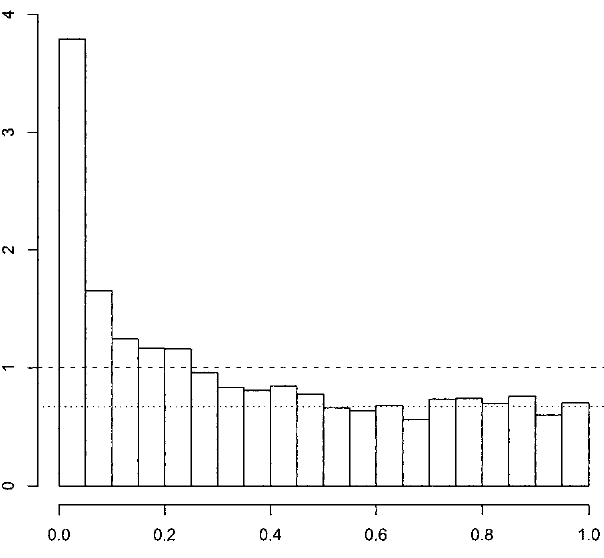
\includegraphics[scale=1.04]{figures/storey-2003-fig1}

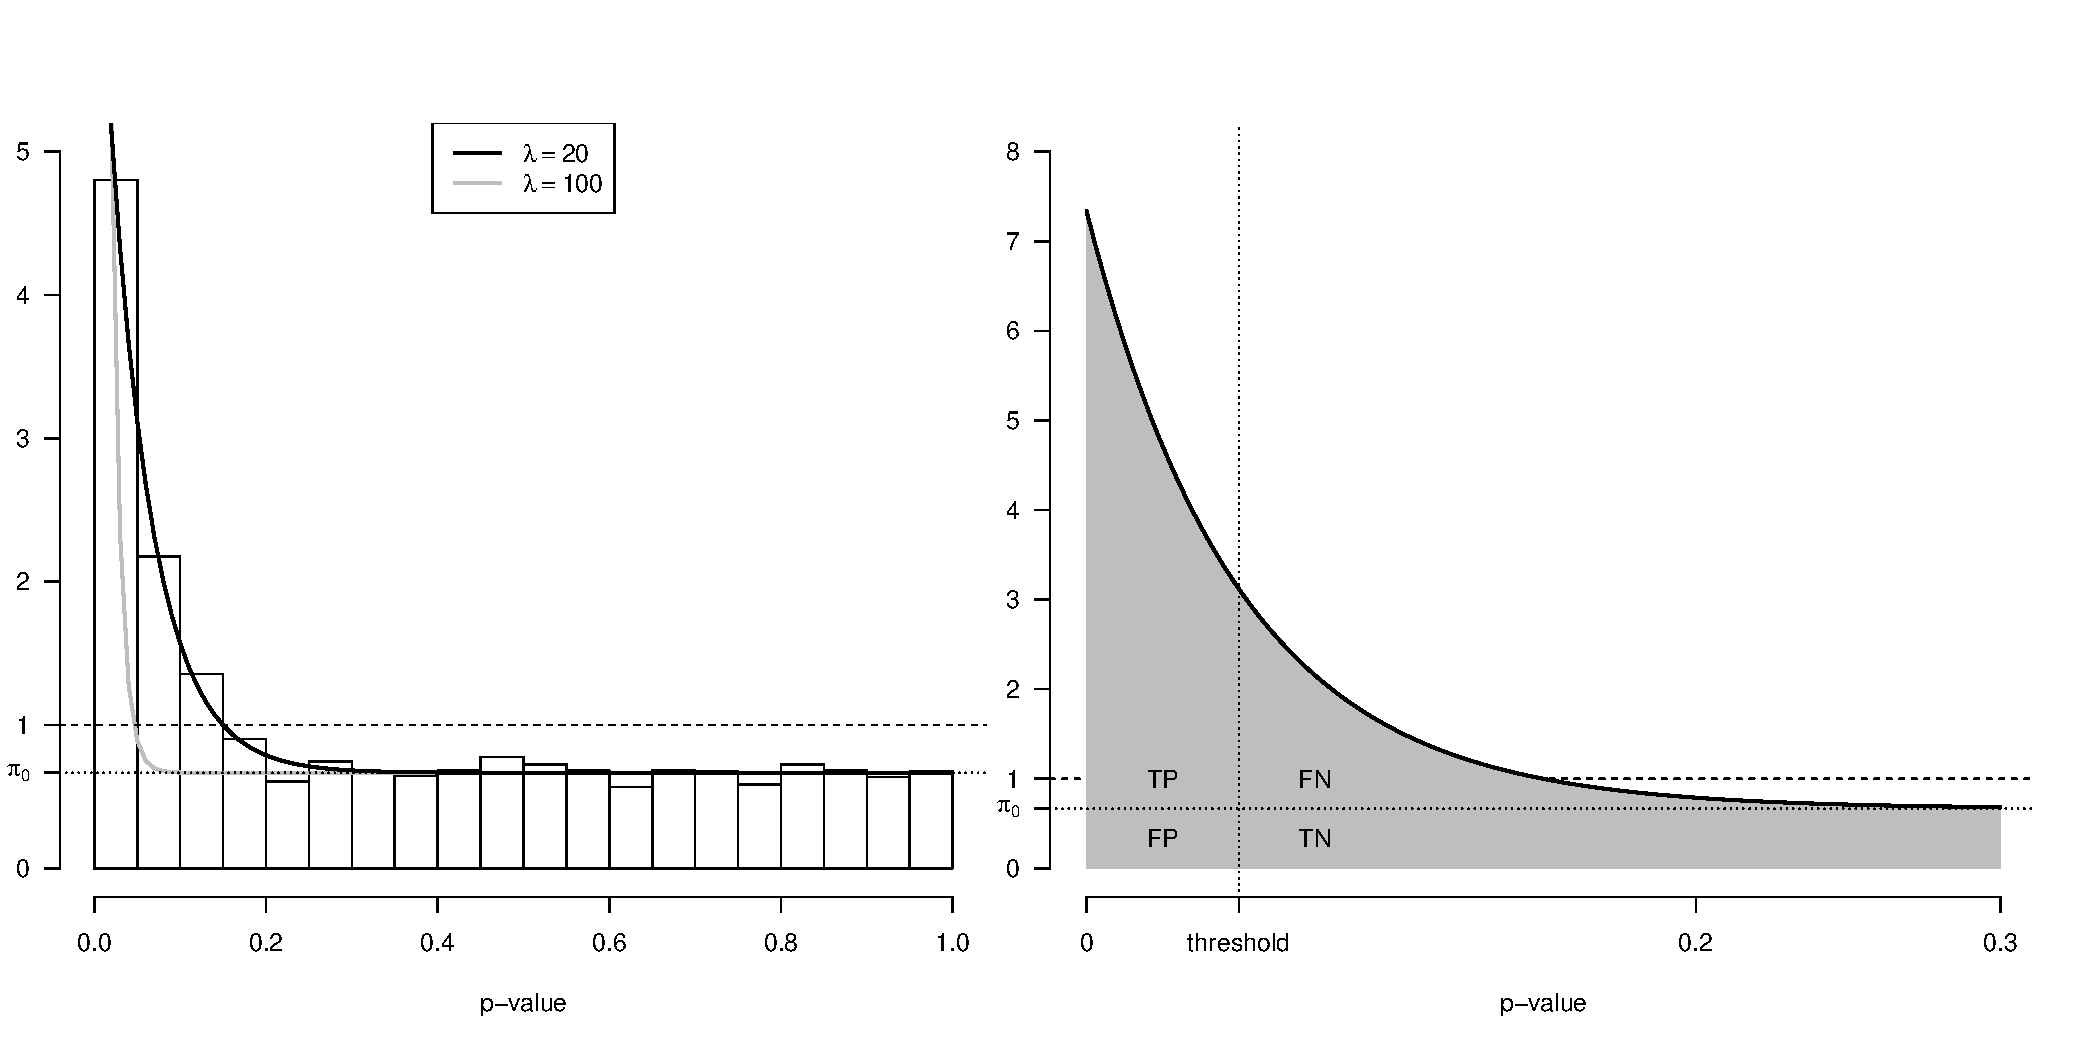
\includegraphics[scale=0.5]{figures/exp-unif-mixture-1.pdf}
\caption{\(\pi_0 : \pi_1\) mixtures of null and alternative distributions of
\(p\)-values.  \emph{Top:} figure taken from ref.~\cite{Storey:2003kx} showing
3170 \(p\)-values from a genomwide study with estimated \(\pi_0 \approx 2/3\).  \emph{Bottom left:} the black and gray thick solid lines show the probability density
function for two mixture distributions defined by
Eq.~\ref{eq:exp-unif-mixture}, with the same \(\pi_0=2/3\) but different \(\lambda\)
values.  The bars correspond to the histogram of a 3170-sized sample from the
``black'' distribution.  \emph{Bottom right:} the same ``black'' distribution
function is expanded to illustrate the four outcomes of hypothesis testing;
their probabilities equal the gray areas delineated by the dotted lines. }
\end{figure}

\begin{table}
\label{tab:fdr-exp-unif-mixture}
\begin{center}
\begin{tabular}{cc|ll|}
 & & \multicolumn{2}{c}{FDR} \\
 \(\lambda\) & threshold \(\alpha\) & \(\pi_1=0.008\) & \(\pi_1=0.052\) \\
\hline
 & \(10^{-2}\) & 0.87 & 0.50 \\
 20 & \(10^{-4}\) & 0.86 & 0.48 \\
 & \(10^{-8}\) & 0.86 & 0.47 \\
\hline
 & \(10^{-2}\) & 0.55 & 0.15 \\
 2000 & \(10^{-4}\) & 0.064 & 0.010 \\
 & \(10^{-8}\) & 0.058 & 0.0090 \\
\hline
\end{tabular}
\end{center}
\caption{False discovery rate calculated using Eq under the mixture distribution
function (Eq.~\ref{eq:exp-unif-mixture}) at various \(\pi_1\) and \(\lambda\) values and various significance
thresholds \(\alpha\).}
\end{table}

\subsection{Calling monoallelic expression}

\begin{equation}
\mathrm{Pr}(\mathrm{TP}) = \pi_1 [1 - (1 - e^{-\lambda}) (e^{-\lambda \alpha} -
e^{-\lambda})]
\end{equation}

\begin{equation}
\mathrm{FDR} = \frac{\mathrm{Pr}(\mathrm{FP})}{\mathrm{Pr}(\mathrm{FP}) + \mathrm{Pr}(\mathrm{TP})}
\end{equation}

\section{More ideal selection}
\label{sec:full-specification}

Scatter plots from the previous analysis indicate that the normal linear model
would not fit well (see
\href{https://docs.google.com/presentation/d/1YvpA1AJ-zzir1Iw0F25tO9x8gkSAzqaO4fjB7K3zBhE/edit?usp=sharing}{Figure
3}).
This qualitative result explains why that work transformed, for each \(g\),
\(\{S_{1g},...,S_{ng}\}\) into percentiles before fitting the normal linear model.  Still before fitting, that analysis averaged
each percentile across 8 selected monoallelically expressed genes, which has a similar effect as
constraining all monoallelically expressed to share parameters
(Eq.~\ref{eq:shared-regression-param})

\bibliography{statistical-overview}

\end{document}
